\documentclass[a5paper, 10pt, twoside]{article}
\usepackage[utf8]{inputenc}
\usepackage[french]{babel}
\usepackage[T1]{fontenc}
\usepackage[top=2cm,bottom=2cm,left=2cm,right=2cm]{geometry}
\usepackage{graphicx}
\usepackage{titlesec}
\usepackage{fontspec}
\usepackage{float}
\usepackage{caption}
\pagenumbering{gobble}

\graphicspath{ {../../static/} {img/} }

\begin{document}
\title{
	{\vspace{3em}\protect\centering\protect
\includegraphics[width=0.9\textwidth]{Pacification_logo}}\\
    {\vspace{4em}\Huge Guide d'utilisateur}\\
	{\large Brainless Devs}
}
\date{
	{\vfill\protect\centering\protect
\includegraphics{brainless_devs.pdf}}\\
}
\maketitle
\cleardoublepage

\section*{Guide d'installation}

Insérez le CD Pacification dans un ordinateur et lancez l'exécutable. Précisez
le lieu d'installation du jeu et suivez les instructions de l'installeur. Ouvrez
l'exécutable de Pacification à l'endroit où vous l'avez installé afin de lancer
le jeu.

\vspace{1cm}

\section*{Guide de désinstallation}

Dans le menu « Démarrer » faites un clic droit sur Pacification, puis choisissez
« Désinstaller ». Cela ouvre le panneau de configuration où vous pouvez
sélectionner puis supprimer le jeu.

\newpage
\section*{Comment jouer ?}

En lançant la partie, vous commencerez sur une map générée aléatoirement, avec
deux unités. Choisissez alors le lieu de fondation de votre première ville avec
le colon, et protégez-vous des ennemis grâce à votre fantassin.\\

Pensez à créer une ville au plus vite en sélectionnant le colon et en appuyant
sur la touche d'action principale lorsqu'il se trouve sur la case souhaitée.\\

Les villes vous permettront de créer de nouvelles unités, et de récolter de
l'argent et de la science à chaque tour. Pensez donc à améliorer les bâtiments
de la ville pour augmenter vos gains, et n'oubliez pas de créer d'autres
unités.\\

Pour assurer le développement de votre empire, vous aurez besoin d'ouvriers
pour exploiter les ressources de la carte, ainsi que construire des routes.\\

Chaque unité d'attaque dispose de ses avantages et de ses inconvénients que
vous découvrirez en jouant. Elles permettent d'attaquer des unités, villes et
ressources ennemies à votre portée. Chaque type d'unité possède des
améliorations qui nécessitent différentes ressources stratégiques, économiques,
et scientifiques.\\

En haut de l'écran, vous trouverez vos différents indicateurs de ressources.
Lorsque vous sélectionnez une ville ou une unité, un menu à droite apparaît
pour vous informer de ses caractéristiques.\\

\begin{figure}[H]
    \centering
    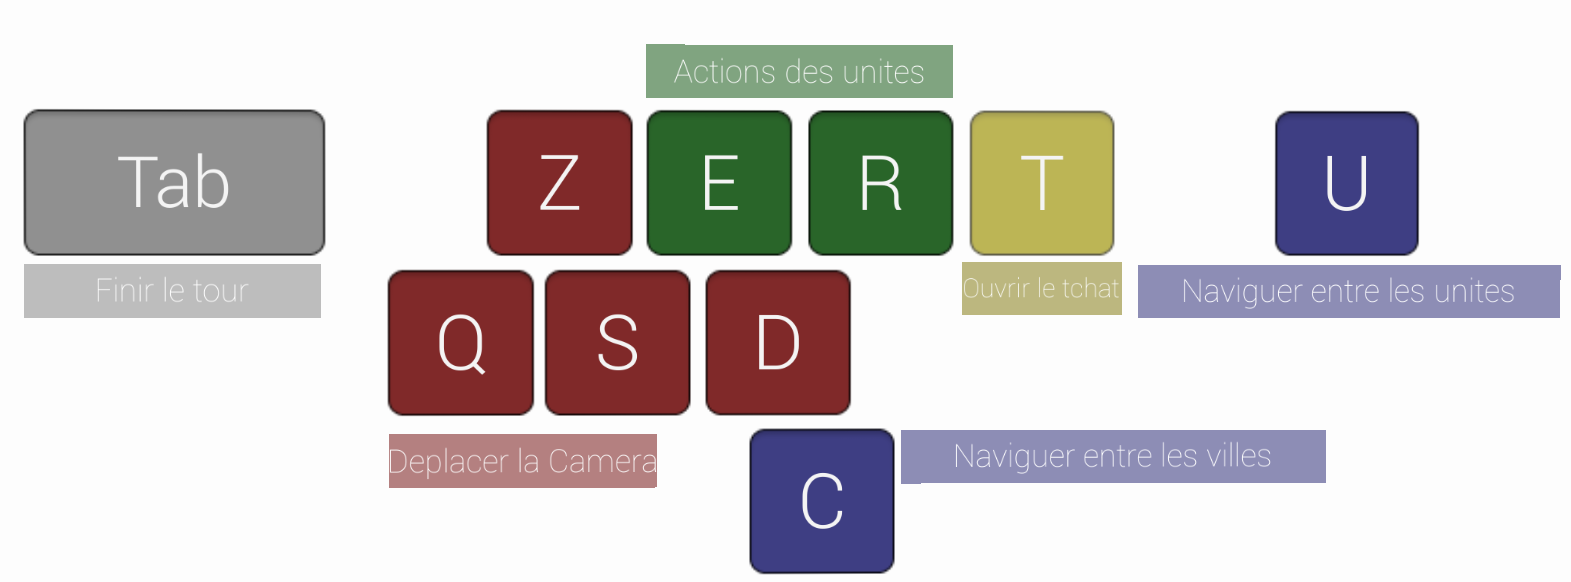
\includegraphics[width=0.95\textwidth]{controls}
\end{figure}

\end{document}
